\documentclass[conference]{IEEEtran}
\IEEEoverridecommandlockouts
% The preceding line is only needed to identify funding in the first footnote. If that is unneeded, please comment it out.
\usepackage{cite}
\usepackage{nth}
\usepackage{amsmath,amssymb,amsfonts}
\usepackage{algorithmic}
\usepackage{graphicx}
\usepackage{textcomp}
\usepackage{xcolor}
\graphicspath{ {./figures/} }

\def\BibTeX{{\rm B\kern-.05em{\sc i\kern-.025em b}\kern-.08em
    T\kern-.1667em\lower.7ex\hbox{E}\kern-.125emX}}
\begin{document}

\title{Conference Paper Title*\\
{\footnotesize \textsuperscript{*}Note: Sub-titles are not captured in Xplore and
should not be used}
\thanks{}
}

\author{\IEEEauthorblockN{1\textsuperscript{st} Given Name Surname}
\IEEEauthorblockA{\textit{dept. name of organization (of Aff.)} \\
\textit{name of organization (of Aff.)}\\
City, Country \\
email address or ORCID}
\and
\IEEEauthorblockN{2\textsuperscript{nd} Given Name Surname}
\IEEEauthorblockA{\textit{dept. name of organization (of Aff.)} \\
\textit{name of organization (of Aff.)}\\
City, Country \\
email address or ORCID}
\and
\IEEEauthorblockN{3\textsuperscript{rd} Given Name Surname}
\IEEEauthorblockA{\textit{dept. name of organization (of Aff.)} \\
\textit{name of organization (of Aff.)}\\
City, Country \\
email address or ORCID}
\and
\IEEEauthorblockN{4\textsuperscript{th} Given Name Surname}
\IEEEauthorblockA{\textit{dept. name of organization (of Aff.)} \\
\textit{name of organization (of Aff.)}\\
City, Country \\
email address or ORCID}
\and
\IEEEauthorblockN{5\textsuperscript{th} Given Name Surname}
\IEEEauthorblockA{\textit{dept. name of organization (of Aff.)} \\
\textit{name of organization (of Aff.)}\\
City, Country \\
email address or ORCID}
\and
\IEEEauthorblockN{6\textsuperscript{th} Given Name Surname}
\IEEEauthorblockA{\textit{dept. name of organization (of Aff.)} \\
\textit{name of organization (of Aff.)}\\
City, Country \\
email address or ORCID}
}

\maketitle

\begin{abstract}
This document is a model and instructions for \LaTeX.
This and the IEEEtran.cls file define the components of your paper [title, text, heads, etc.]. *CRITICAL: Do Not Use Symbols, Special Characters, Footnotes, 
or Math in Paper Title or Abstract.
\end{abstract}

\begin{IEEEkeywords}
component, formatting, style, styling, insert
\end{IEEEkeywords}

\section{Introduction}
Modern day digital cameras involve the use of image sensor array, with millions of pixels. Although it can achieve high resolution, imaging it has many downsides, as more megapixels require more image processing power during image acquisition. However, it is possible to take images using only a single pixel from a single photo-diode instead of an array of pixels. Moreover this type of imaging technique can be applied for capturing images at wavelengths that are outside the range of general camera sensor arrays.\par
This enables us to greatly simplify the general camera architecture, all the while reducing costs. Single pixel imaging involves modulating the light by a digital micro mirror device or a programmable light modulator. The photo-diode receives the correlated light from which image can be reconstructed using compressive sensing algorithms and machine learning models.\par
In this paper we review a wide range of single pixel imaging techniques and compare their performance in various settings, compare their performance with respect to the reconstructed image size and the noise level in terms of reconstruction power and time taken. Finally, we conclude by presenting a deep learning approach on reconstructed images via single pixel imaging techniques to make high-resolution RGB images.

\section{Related Works}

\subsection{subsection}
-----------
\section{Background}
Single pixel imaging is a novel technique for computational imaging. Although high resolution digital cameras are used in mainstream, it is quite challenging to capture high quality images, especially in noisy illuminated environmental conditions. Moreover images can be reconstructed from data captured by a single photo detector even without direct line of site.\par
This technique is quite similar to compressive sensing, thus an image can be reconstructed even from sub-Nyquist measurements.
In this paper we experimentally obtain high resolution RGB images from a single channel photo detector by applying reconstruction algorithms and deep learning\par

\begin{figure}[h]
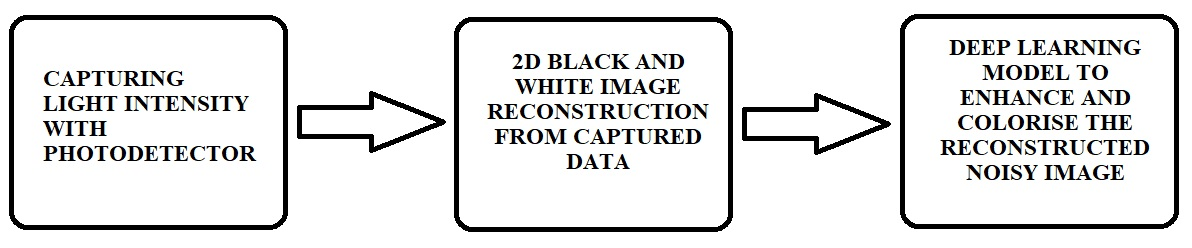
\includegraphics[scale=0.34]{figures/flow diagram.jpg}
\caption{Flow diagram for Image reconstruction with SPI}
\label{fig:flow_diagram}
\end{figure}

Fig:\ref{fig:flow_diagram}, shows the flow diagram for our system from capturing light with the photo detector and reconstructing image by a reconstruction algorithm, followed by deep learning model.


\par Single pixel imaging results in a low signal- to –noise ratio (SNR) and thus poor image quality. We propose a deep learning model to enhance the image to obtain greater SNR and color images with high resolution.
\subsection{Principle}\label{AA}
In SPI, spatial information is modulated by using an SLM and specific patterns to encode image information spatially into 1-D light signals.Structured patterns are displayed on the SLM and the patterns are projected onto the object to be imaged.\par
The light detected by the photodetector is the intensity of the resulting light transmitted, reflected or fluorescence by the object to be imaged.
\par
The light intensity detected by the photodetector is closely related to the reflected light and the projected pattern by the photodetector can be depicted by the eq: 
\begin{equation}D{i}=a\sum_{x=1}^{M}\sum_{y=1}^{N}O(x,y).P{i}(x,y)\end{equation}
\par
(x,y)  is the spatial coordinate. The reflectivity is denoted by O, $i$\textsuperscript{$th$} structured pattern is denoted by $P$\textsubscript{$i$}, $a$ is a constant factor dependant on the optoelectronic property of the used single pixel detector. The size of both $O$ and $Pi$ is $M$ x $N$ pixels.

\begin{figure}[h]
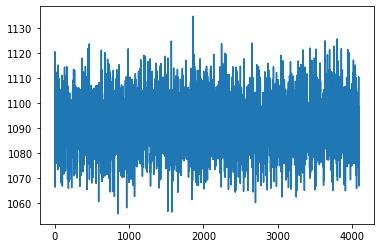
\includegraphics[scale=0.66]{figures/measurements_graph.png}
\caption{Measurements for Single Pixel Imaging}
\label{fig:measurements_graph}
\end{figure}

Fig:\ref{fig:measurements_graph} shows the single pixel measurements after spatial light modulation.
\par The image reconstructed from the single pixel measurements by the reconstruction algorithms is proportional to object reflectivity O. Eq:-- depicts the relationship among single pixel measurements, pattern structures and the reconstructed object.
\par
Spatial light modulation can be achieved in two different ways, first, the structured detection scheme and second, the structured illumination scheme
\par The single pixel detection methods mainly falls into three categories: \begin{itemize}
\item[1]structure pattern types used in spatial light modulation
\item[2]strategy of sampling
\item[3]image reconstruction algorithm
\end{itemize}

\par In our paper we perform a quantitative comparison among various reconstruction algorithms and apply a deep learning approach for obtaining high resolution color(RGB) images after image reconstruction,

\subsection{Image Reconstruction algorithms}
\begin{itemize}
\item Non Iterative Methods:
    \begin{itemize}
        \item Basis scan
        \smallskip
        \par Basis scan algorithm reconstructs images from N light measurements from various combinations of pixels, by utilizing test functions from general basis.
        \par
        Hadamard basis can be used for reconstrutcting images from single pixel measurements as demonstrated by Duarte et al.[]. Hadamard patterns  are orthogonal with binary values +1 or -1. 
        \begin{equation}
            H_{2}=\begin{bmatrix}
            1&1 \\ 
            1&-1 
            \end{bmatrix}
        \end{equation}
            H2 is the initial matrix from which the Hadamard matrix can be derived. 
        \begin{equation}
            H_{2}=\begin{bmatrix}
            H_{2}k-1&H_{2}k-1 \\ 
            H_{2}k-1&-H_{2}k-1 
            \end{bmatrix}
        \end{equation}    
        \par For a N pixel image, imaging masks are created by using Hadamard matrix of size $N$x$N$.\par Final reconstructed image can be obtained by a product of the Hadamard matrix and the vector $S$ of detected signals. The result is a one-dimensional vector of the output image $O$.
        \begin{equation}
            O=H.S
        \end{equation} 
        The final reconstructed image can be obtained by reshaping the one-dimensional vector O to a two-dimensional image
        
        \begin{figure}[!h]
               \centering
             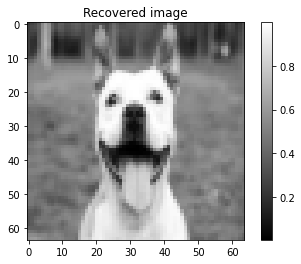
\includegraphics[scale=0.6]{figures/basis_scan_normal.png}
                \caption{Reconstructed image using Basis Scan algorithm}
        \label{fig:basis_scan_normal}
        \end{figure}
        
        The image reconstructed using basis scan algorithm is shown in Fig:\ref{fig:basis_scan_normal} with 1x sampling ratio for a 64x64 image with 4096 measurements.
        \medskip
        \item Correlation Modulation Method
        \smallskip
        \par Single pixel imaging utilizes the correlation between the modulating patterns and the actual scene. By the correlation modulation method, the image can be reconstructed by correlating modulating patterns with detected light measurements.
        \begin{equation}
            X=\left \{ b_{i}a_{i} \right \}-\left \{ b_{i}\right \}\left \{ a_{i}\right \}
        \end{equation}
        $X$ denotes the reconstructed image obtained by correlating between modulation patterns and measured light intensity values. \par The $i$\textsuperscript{$th$} column in the measurement is denoted by $b$\textsubscript{i} and the $i$\textsuperscript{$th$} row in the modulation matrix is denoted by $a$\textsubscript{$i$}
        
         \begin{figure}[h]
               \centering
             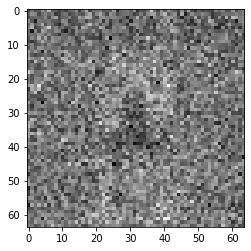
\includegraphics[scale=0.6]{figures/correlation_modulation.png}
                \caption{Reconstructed image using Correlation Modulation algorithm}
        \label{fig:correlation_modulation_normal}
        \end{figure}
        \par Fig:\ref{fig:correlation_modulation_normal} shows the reconstructed image using correlation modulation method.
        \medskip
        
        \item Differential Ghost Imaging
        \smallskip
        \par This method is an improvement to the correlation modulation method by taking into account the fluctuation in illumination.
        \begin{equation}
            X=\left \{ b_{i}a_{i} \right \}-\frac{\left \{ b_{i} \right \}}{\left \{a_{i} \right \}}\left \{ s_{i}a_{i} \right \}
        \end{equation}
        where $X$ is the reconstructed image and $s$ \(\in\) R\textsuperscript{$m$ x $l$}
        
        \begin{figure}[!h]
               \centering
             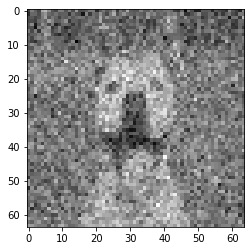
\includegraphics[scale=0.6]{figures/differential_ghost_imaging.png}
                \caption{Reconstructed image using Differential Ghost Imaging algorithm}
        \label{fig:differential_ghost_imaging_normal}
        \end{figure}
        \par
        The image reconstructed using differential ghost Imaging method is shown in Fig:\ref{fig:differential_ghost_imaging_normal}
    \end{itemize}
    \bigskip
    \item Iterative Methods:
        \begin{itemize}
            \item Gradient Descent
            \smallskip
            \par The SPI image reconstruction can be formulated as a error minimization problem, where the goal is to reduce the error between real and estimated measurements.
            \begin{equation}
                min_{xL}(x)=min_{x}\left \| Ax-b \right \|l_{2}^2
            \end{equation}
            Where \(l_{2}\) norm is defined as \(\left \| x \right \|_{l_{2}}=\sqrt{\sum_{i}(x_{i}^2)}\) .The image can be reconstructed iteratively by updating x as 
            \begin{equation}
                {x}'=x-\triangle_{x}p
            \end{equation}
            \par where \(\triangle_{x}\) denotes the step size and p denotes the gradient as \(p=\frac{\partial L(x)}{\partial x}=2A^T(Ax-b)\).
            Updation process is converged when the objective function becomes smaller than a given threshold value.
            
            \begin{figure}[!h]
               \centering
             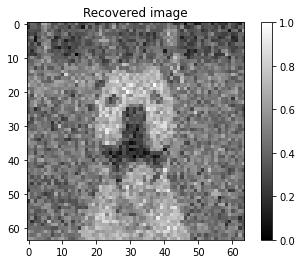
\includegraphics[scale=0.6]{figures/gradient_descent.png}
                \caption{Reconstructed image using Differential Ghost Imaging algorithm}
        \label{fig:gradient_descent_normal}
        \end{figure}
            
            \par The reconstructed image from raw measurements by gradient descent method is shown in Fig:\ref{fig:gradient_descent_normal}
            \bigskip
        \item Conjugate Gradient Descent
        \par Similar to the Gradient Descent algorithm, CGD also solves the quadratic minimization problem ,but A must be symmetric and positive.
        \begin{equation}
            A^TAx=A^{Tb}\Leftrightarrow {A}'x={b}'
        \end{equation}
        \par Where \({A}' \in R^{n x n}\) and \({b}' \in R^{n x n}=A^Tb\) Residual error vector is denoted by
        \begin{equation}
            r^{(k)}={b}'-{A}'x^{(k)}=A^TAx^{(k)}
        \end{equation}
        while gradient is defined as
        \begin{equation}
            p^{(k)}=-r^{(k-1)}-\frac{r^{(k-1)T}r^{(k-1)}}{r^{(k-2)T}r^{(k-2)}}p^{(k-1)}
        \end{equation}
        where $k$ denotes the residual error vector at the iteration k. Optimum step size can be obtained by the equation
        \begin{equation}
            \triangle_{x}^{(k)}=\frac{r^{(k-1)T}r^{(k-1)}}{p^{(k)T}{A}'p^{(k)}}
        \end{equation}
        
        
        The main advantage of CGD over gradient descent is that the former has faster convergence (no more than n iterations for an n-pixel image)as compared to the latter, the reason being conjugate gradients in each iteration.
        \par Fig:\ref{fig:conjugate_gradient_descent_normal} shows the image reconstructed by Conjugate gradient descent algorithm, converged in 210 iterations with 0.00098 as the RMSE error.
        \begin{figure}[ht]
               \centering
             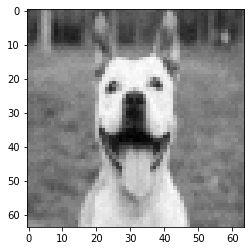
\includegraphics[width=0.6\linewidth]{figures/conjugate_gradient_descent.png}
                \caption{Reconstructed image using Conjugate Gradient Descent algorithm}
        \label{fig:conjugate_gradient_descent_normal}
        \end{figure}
        \end{itemize}
\end{itemize}

\subsection{Simulation}
\par The comparison among the five SPI reconstruction algorithms are done by numerical simulation from the aspects of sampling ratio and reconstruction error, image size and noises level. The reconstruction error on these images are averaged to quantitatively measure each algorithm.We use the image of “cameraman” to perform SPI reconstruction. Random modulation is applied to synthesize measurements.
\par The simulations are implemented on a computer with intel core i5 9th gen processor, 8gb RAM and python 3.7.

\subsection{Quantitative Comparison }
\par For the comparison among various algorithms, we test our algorithms based on normalized root mean square error (RMSE) and compare their performance with respect to sampling ratio, noise level influence and image size.\par
Normalized RMSE is defined as the relative difference between ground truth and reconstructed image.
\begin{equation}
    RMSE=\sqrt{\frac{\left \{ (l_{1}-l_{2})^2 \right \}}{\left \{ I_{1} \right \}}}
\end{equation}
where $I_{1}$ denotes the ground truth image and $I_{2}$ denotes the image reconstructed by SPI algorithms.
\begin{itemize}
    \item Sampling Ratio
    \medskip
    \par The normalized RMSE for the five reconstruction algorithms are calculated for sampling ratios ranging from 0.5 to 5.0. \par
	Sampling ratio is defined as the ratio between number of measurements to the number of pixels in ground truth image. The reconstructed image of original image is shown below for each algorithm along with reconstruction error.
        \begin{figure}[ht]
        \centering
        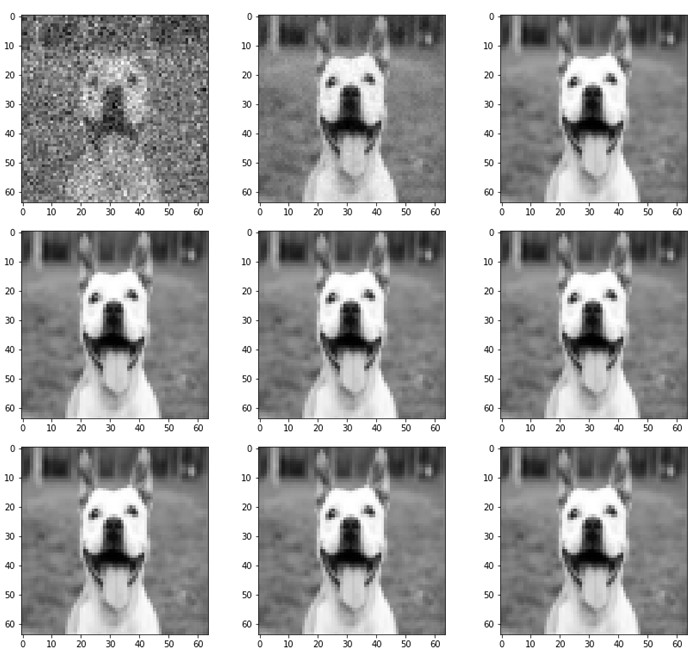
\includegraphics[scale=0.55]{figures/cgd_sampling_ratio.jpg}
        \caption{Reconstructed images using Conjugate Gradient Descent for sampling ratios ranging 0.5 - 4.5}
        \label{fig:cgd_sampling_ratio}
        \end{figure}
    \par Fig:\ref{fig:cgd_sampling_ratio} shows the reconstructed images for conjugate gradient descent algorithm for sampling ratios ranging from 0.5 to 4.5 in steps of 0.5.
    \begin{figure}[ht]
        \centering
        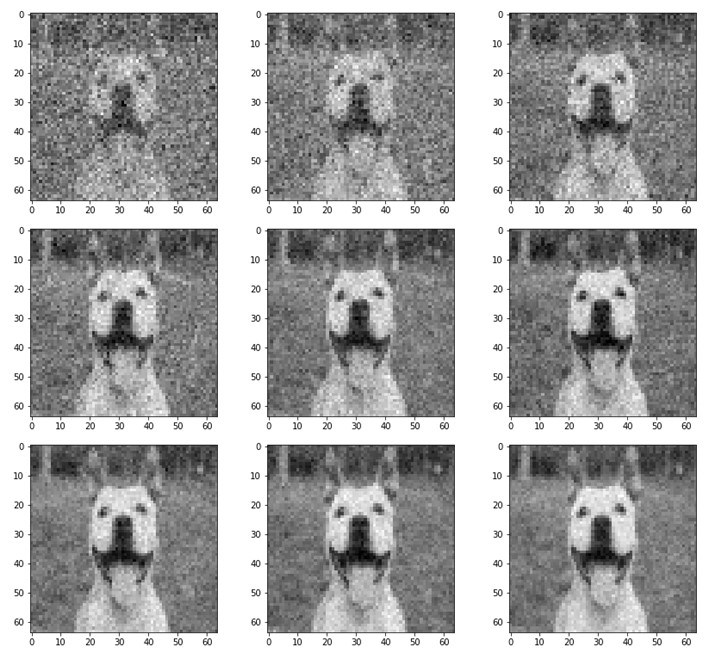
\includegraphics[scale=0.55]{figures/gd_sampling_ratio.jpg}
        \caption{Reconstructed images using Gradient Descent for sampling ratios ranging 0.5 - 4.5}
        \label{fig:gd_sampling_ratio} 
        
        \end{figure}
    \par Fig:\ref{fig:gd_sampling_ratio} shows the reconstructed images for gradient descent algorithm for sampling ratios ranging from 0.5 to 4.5 in steps of 0.5.
    \bigskip
    \bigskip
    \bigskip
    \bigskip
    \begin{figure}[ht]
        \centering
        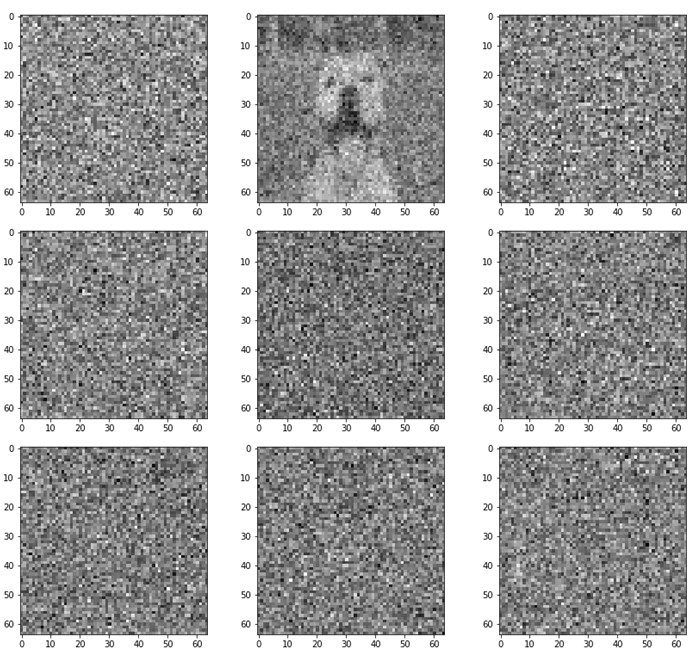
\includegraphics[scale=0.55]{figures/dgi_sampling_ratio.jpg}
        \caption{Reconstructed images using Differential Ghost Imaging for sampling ratios ranging 0.5 - 4.5}
        \label{fig:dgi_sampling_ratio}
        \end{figure}
    \par Fig:\ref{fig:dgi_sampling_ratio} shows the reconstructed images for Differential Ghost Imaging algorithm for sampling ratios ranging from 0.5 to 4.5 in steps of 0.5.
    
    \begin{figure}[ht]
        \centering
        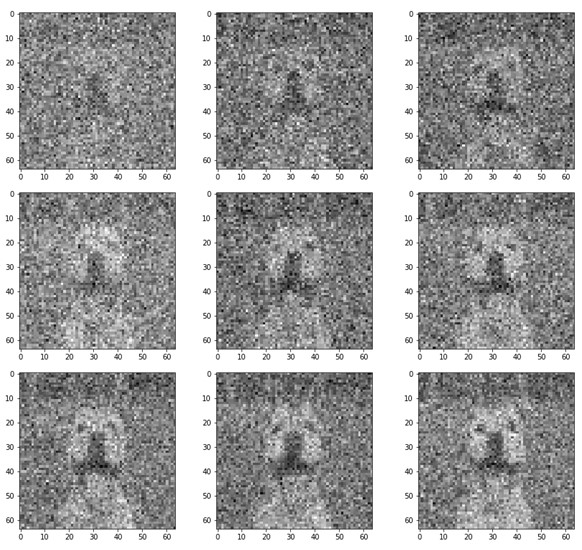
\includegraphics[scale=0.65]{figures/cm_sampling_ratio.jpg}
        \caption{Reconstructed images using Correlation Modulation method for sampling ratios ranging 0.5 - 4.5}
        \label{fig:cm_sampling_ratio}
        \end{figure}
    \par Fig:\ref{fig:cm_sampling_ratio} shows the reconstructed images for Correlation Modulation method algorithm for sampling ratios ranging from 0.5 to 4.5 in steps of 0.5.
    \bigskip
    \bigskip
    \bigskip
    \bigskip
    \bigskip
    \begin{figure}[ht]
        \centering
        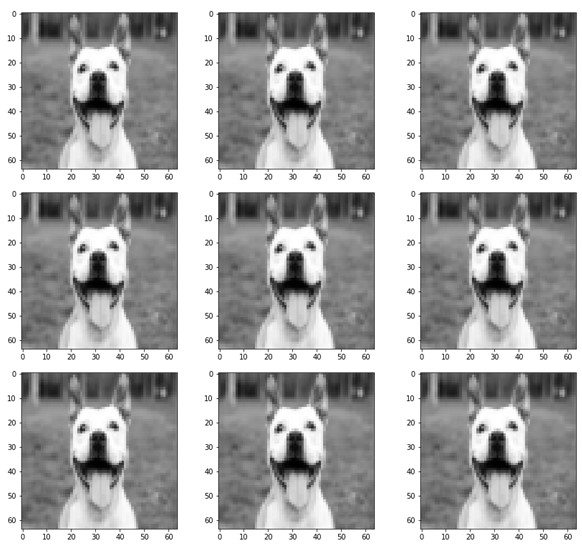
\includegraphics[scale=0.65]{figures/basisScan_sampling_ratio.jpg}
        \caption{Reconstructed images using basis scan algorithm for sampling ratios ranging 0.5 - 4.5}
        \label{fig:basisScan_sampling_ratio}
        \end{figure}
    \par Fig:\ref{fig:basisScan_sampling_ratio} shows the reconstructed images for basis scan algorithm for sampling ratios ranging from 0.5 to 4.5 in steps of 0.5.
    
    \begin{figure}[ht]
        \centering
        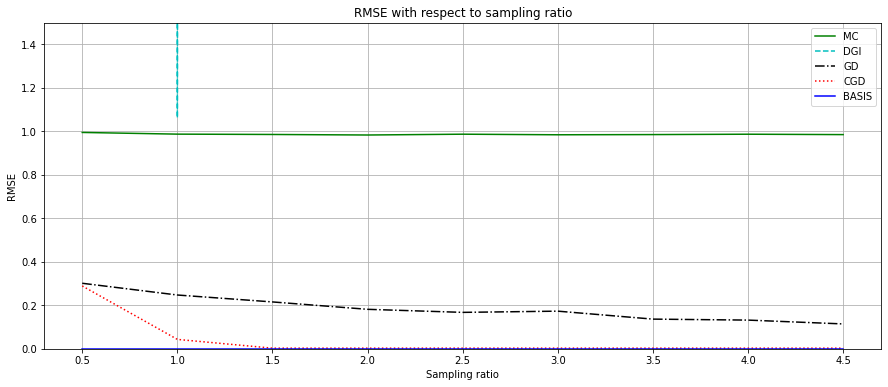
\includegraphics[scale=0.27]{figures/sampling_ratio_RMSE.png}
        \caption{Root Mean Square Error(RMSE) versus sampling ratio plot for the different image reconstruction algorithms}
        \label{fig:sampling_ratio_RMSE}
        \end{figure}
    \par Fig:\ref{fig:sampling_ratio_RMSE} shows the RMSE vs Sampling ratio plot for different reconstruction algorithms for sampling ratios ranging from 0.5 to 4.5 in steps of 0.5.
    \par From Fig:\ref{fig:sampling_ratio_RMSE}, it is evident that the best result is achieved by basis scan algorithm but the CGD algorithm performs better overall in terms of RMSE and time taken to converge. The gradient descent algorithm also performed well but the differential ghost imaging and Correlation modulation method performed poorly as far as RMSE and convergence time is concerned.
    \bigskip
    \item Noise Level
    \medskip \par
    For simulating noise level influence on different algorithms we add Gaussian white noise which is in par with real life measurements which are always full of noise from sources like ambient light.
    The Gaussian noise probability distribution is shown in Eq. :\ref{eq:gaussian noise equation}
    \begin{equation}
    \label{eq:gaussian noise equation}
        P(N)=\frac{1}{\sqrt{2\pi\sigma}}\exp{\left(-\frac{N^2}{2\sigma^2}\right)}
    \end{equation}
    \par Where noise is defined by \(N\) and \(\sigma\) is the standard deviation.
    \par We consider the ratios \(1{e}^-4\), \(5{e}^-4\) and \(3{e}^-3\) to generate the noise while keeping a constant image size of 64x64 pixels and constant sampling ratio of 1.The reconstructed images from various reconstruction algorithms are shown below.
    
     \begin{figure}[ht]
        \centering
        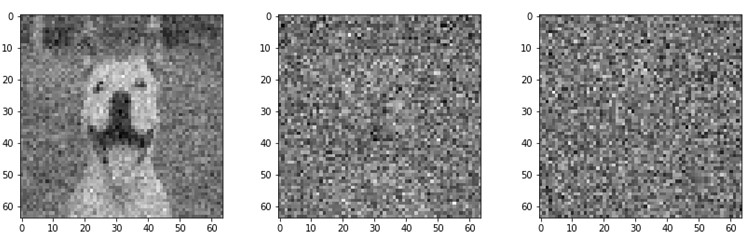
\includegraphics[scale=0.55]{figures/cgd_noise_influence.jpg}
        \caption{Reconstructed images using conjugate gradient descent for Noise levels of \(1{e}^{-4}\), \(5{e}^{-4}\) and \(3{e}^{-3}\) respectively}
        \label{fig:cgd_noise_influence}
        \end{figure}
    \par Fig:\ref{fig:cgd_noise_influence} shows the reconstructed images for conjugate gradient descent algorithm for noise levels of \(1{e}^{-4}\), \(5{e}^{-4}\) and \(3{e}^{-3}\).
    
    \begin{figure}[ht]
        \centering
        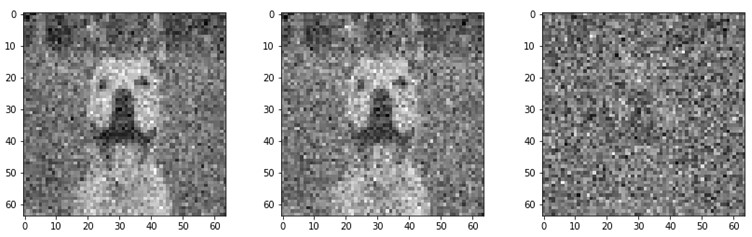
\includegraphics[scale=0.55]{figures/gd_noise_influence.jpg}
        \caption{Reconstructed images using gradient descent for Noise levels of \(1{e}^{-4}\), \(5{e}^{-4}\) and \(3{e}^{-3}\) respectively}
        \label{fig:gd_noise_influence}
        \end{figure}
    \par The reconstructed images using gradient descent algorithm for noise levels of \(1{e}^{-4}\), \(5{e}^{-4}\) and \(3{e}^{-3}\) respectively are shown in Fig:\ref{fig:gd_noise_influence}.
    
    \begin{figure}[ht]
        \centering
        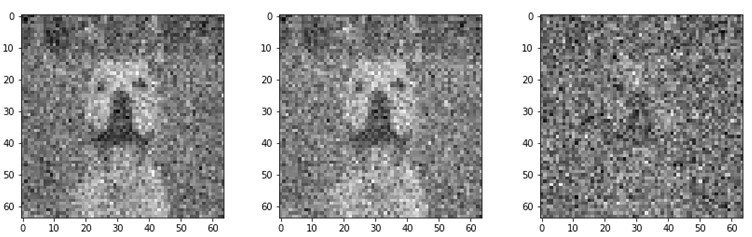
\includegraphics[scale=0.55]{figures/dgi_noise_influence.jpg}
        \caption{Reconstructed images using differential ghost imaging for Noise levels of \(1{e}^{-4}\), \(5{e}^{-4}\) and \(3{e}^{-3}\) respectively}
        \label{fig:dgi_noise_influence}
        \end{figure}
    \par The reconstructed images using differential ghost imaging algorithm for noise levels of \(1{e}^{-4}\), \(5{e}^{-4}\) and \(3{e}^{-3}\) respectively are shown in Fig:\ref{fig:dgi_noise_influence}.
    \bigskip\bigskip\bigskip
    \begin{figure}[ht]
        \centering
        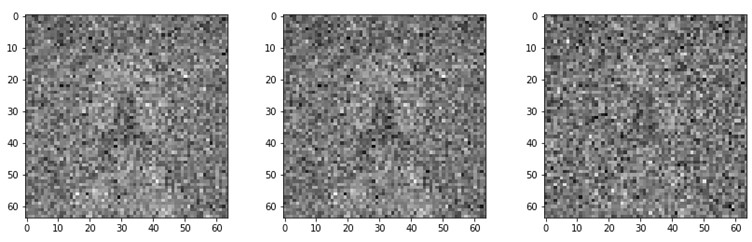
\includegraphics[scale=0.55]{figures/correlationModulation_noise_influence.jpg}
        \caption{Reconstructed images using Correlation Modulation algorithm for Noise levels of \(1{e}^{-4}\), \(5{e}^{-4}\) and \(3{e}^{-3}\) respectively}
        \label{fig:cm_noise_influence}
        \end{figure}
    \par The reconstructed images using differential Correlation Modulation algorithm for noise levels of \(1{e}^{-4}\), \(5{e}^{-4}\) and \(3{e}^{-3}\) respectively are shown in Fig:\ref{fig:cm_noise_influence}.
    
    \begin{figure}[ht]
        \centering
        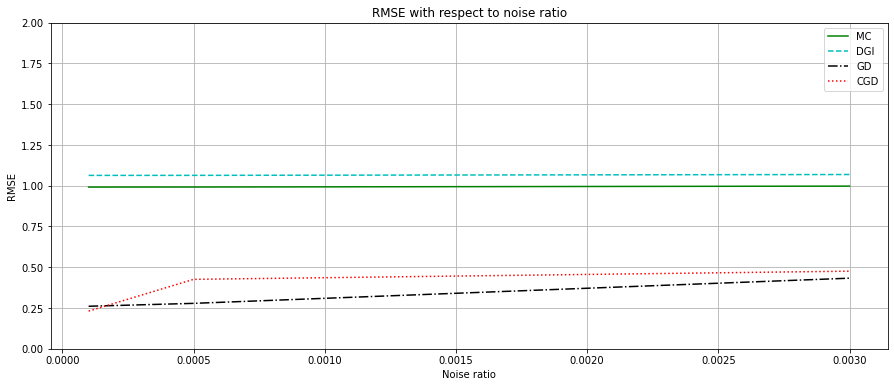
\includegraphics[scale=0.27]{figures/noise_ratio_RMSE.png}
        \caption{Root Mean Square Error(RMSE) versus Noise ratio plot for the different image reconstruction algorithms}
        \label{fig:noise_ratio_RMSE}
        \end{figure}
    \par Fig:\ref{fig:noise_ratio_RMSE} shows the RMSE vs Noise ratio plot for different reconstruction algorithms for noise ratios of \(1{e}^{-4}\), \(5{e}^{-4}\) and \(3{e}^{-3}\) with a constant sampling ratio of 1 and constant image size of 64x64.
    \par From Fig:\ref{fig:noise_ratio_RMSE}, it is evident that the best result is achieved by the Gradient descent algorithm in terms of RMSE. CGD comes second in terms of RMSE but it takes less time taken to converge. The differential ghost imaging and Correlation modulation method performed poorly as far as RMSE and convergence time is concerned.
\end{itemize}



\subsection{Deep Learning Approach}
So far, among all the different algorithms conjugate gradient descent really stood out for lower absolute Root mean squared error, faster convergence and higher noise immunity.All our experiments has been so far with grayscale images. Conventionally for obtainging colored RGB SPI images RGB sensors are required, which substantially increase sampling time for a image scene. In order to improve sampling time and increase resolution in SPI images we propose a deep learning approach to obtain high resolution RGB images even from a grayscale single pixel detector.
In our approach, we first reconstruct the grayscale SPI image with CGD algorithm, then apply a deep GAN model to upsample and colorize the reconstructed low resolution grayscale image.

\subsubsection{Dataset Generation}
\par For training the Generative adversarial network, SPI reconstructed image is needed as input to the mode. Input images are grayscale  64x64 pixel images.
Conjugated gradient descent algorithm has been chosen for generating input images by reconstructing 64 x64 pixel grayscale images from single pixel detector measurements, which are synthesized by random modulation method This algorithm has been chosen because it had a very good performance among other algorithms.
The NYU V2 dataset’s indoor colored high resolution images has been used as the target image for training and testing the model. Due to hardware limitations the original images are resized to 256x256 rgb images, which are then used to generate SPI reconstructed image by CGD algorithm.
\begin{figure}
\centering
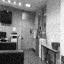
\includegraphics[width=.3\linewidth]{figures/input_spi_image.png} % Just stack two includegraphics!
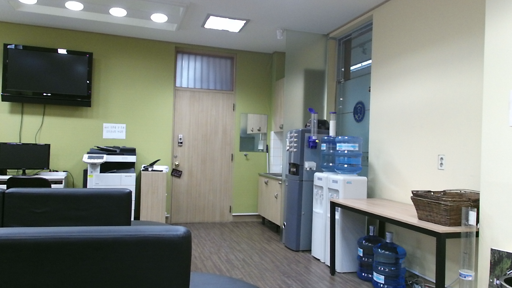
\includegraphics[width=.535\linewidth]{figures/output_color_image.png}
\caption{SPI input image and color output image for Deep learning model}
\label{fig:deep_learning_model_sample_image}
\end{figure}
\par
Fig.:\ref{fig:deep_learning_model_sample_image} shows an example input image and corresponding high resolution color image respectively.
\medskip
\subsubsection{Training and Testing}
The synthesized dataset containing 2000 images has been divided in 8:2 as training and testing samples. The model has been trained on Intel® Xeon(R) Silver 4210 CPU @ 2.20GHz × 40 with Tesla v100 GPU and Linux Centos 7 Gnome version 3.28.2 hardware.
The following figures shows the training and testing accuracy of the generator and the discriminator model of the GAN.
The fully trained generator network has an accuracy of -- as shown in fig:
\medskip
\subsubsection{Deep Learning Model}
\par We propose a deep learning model to obtain high quality, up-scaled, RGB images from low quality images reconstructed by Conjugate gradient descent algorithm. This is implemented by an generative adversarial network (SRGAN---) which is pretrained by simulated reconstructed images. 

\begin{figure}[ht]
\centering
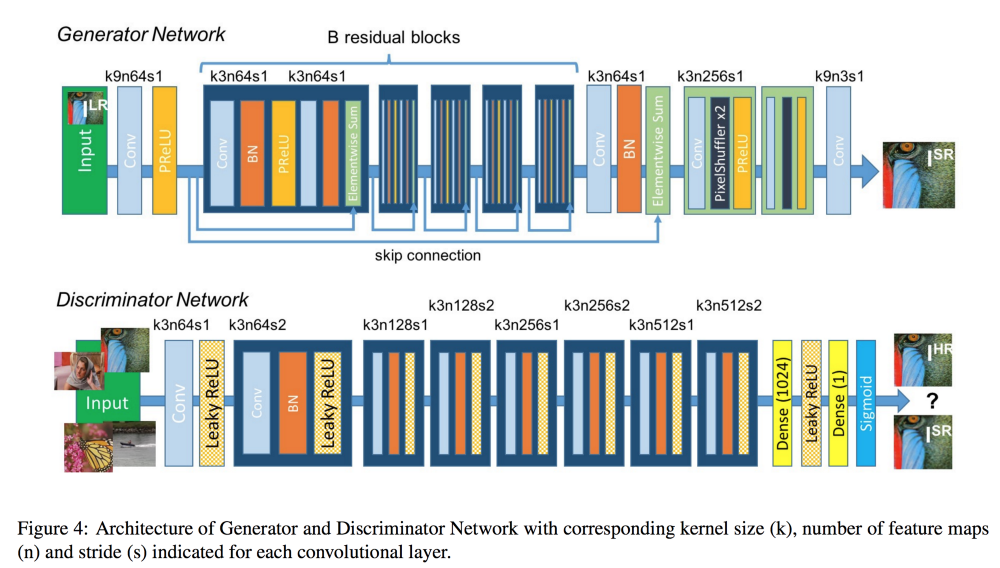
\includegraphics[width=1\linewidth]{figures/srgan_architecture.png} % Just stack two includegraphics!
\caption{Framework of SRGAN for RGB image reconstruction from SPI images}
\label{fig:deep_learning_model_sample_image}
\end{figure}
\par
Fig.:\ref{fig:deep_learning_model_sample_image} shows the architechture of SRGAN, consisting of two parts: generator network and discriminator network.
\medskip

\subsection{Identify the Headings}
Headings, or heads, are organizational devices that guide the reader through 
your paper. There are two types: component heads and text heads.

Component heads identify the different components of your paper and are not 
topically subordinate to each other. Examples include Acknowledgments and 
References and, for these, the correct style to use is ``Heading 5''. Use 
``figure caption'' for your Figure captions, and ``table head'' for your 
table title. Run-in heads, such as ``Abstract'', will require you to apply a 
style (in this case, italic) in addition to the style provided by the drop 
down menu to differentiate the head from the text.

Text heads organize the topics on a relational, hierarchical basis. For 
example, the paper title is the primary text head because all subsequent 
material relates and elaborates on this one topic. If there are two or more 
sub-topics, the next level head (uppercase Roman numerals) should be used 
and, conversely, if there are not at least two sub-topics, then no subheads 
should be introduced.

\subsection{Figures and Tables}
\paragraph{Positioning Figures and Tables} Place figures and tables at the top and 
bottom of columns. Avoid placing them in the middle of columns. Large 
figures and tables may span across both columns. Figure captions should be 
below the figures; table heads should appear above the tables. Insert 
figures and tables after they are cited in the text. Use the abbreviation 
``Fig.~\ref{fig}'', even at the beginning of a sentence.

\begin{table}[htbp]
\caption{Table Type Styles}
\begin{center}
\begin{tabular}{|c|c|c|c|}
\hline
\textbf{Table}&\multicolumn{3}{|c|}{\textbf{Table Column Head}} \\
\cline{2-4} 
\textbf{Head} & \textbf{\textit{Table column subhead}}& \textbf{\textit{Subhead}}& \textbf{\textit{Subhead}} \\
\hline
copy& More table copy$^{\mathrm{a}}$& &  \\
\hline
\multicolumn{4}{l}{$^{\mathrm{a}}$Sample of a Table footnote.}
\end{tabular}
\label{tab1}
\end{center}
\end{table}

\begin{figure}[htbp]
\caption{Example of a figure caption.}
\label{fig}
\end{figure}

Figure Labels: Use 8 point Times New Roman for Figure labels. Use words 
rather than symbols or abbreviations when writing Figure axis labels to 
avoid confusing the reader. As an example, write the quantity 
``Magnetization'', or ``Magnetization, M'', not just ``M''. If including 
units in the label, present them within parentheses. Do not label axes only 
with units. In the example, write ``Magnetization (A/m)'' or ``Magnetization 
\{A[m(1)]\}'', not just ``A/m''. Do not label axes with a ratio of 
quantities and units. For example, write ``Temperature (K)'', not 
``Temperature/K''.

\section*{Acknowledgment}

The preferred spelling of the word ``acknowledgment'' in America is without 
an ``e'' after the ``g''. Avoid the stilted expression ``one of us (R. B. 
G.) thanks $\ldots$''. Instead, try ``R. B. G. thanks$\ldots$''. Put sponsor 
acknowledgments in the unnumbered footnote on the first page.

\section*{References}

Please number citations consecutively within brackets \cite{b1}. The 
sentence punctuation follows the bracket \cite{b2}. Refer simply to the reference 
number, as in \cite{b3}---do not use ``Ref. \cite{b3}'' or ``reference \cite{b3}'' except at 
the beginning of a sentence: ``Reference \cite{b3} was the first $\ldots$''

Number footnotes separately in superscripts. Place the actual footnote at 
the bottom of the column in which it was cited. Do not put footnotes in the 
abstract or reference list. Use letters for table footnotes.

Unless there are six authors or more give all authors' names; do not use 
``et al.''. Papers that have not been published, even if they have been 
submitted for publication, should be cited as ``unpublished'' \cite{b4}. Papers 
that have been accepted for publication should be cited as ``in press'' \cite{b5}. 
Capitalize only the first word in a paper title, except for proper nouns and 
element symbols.

For papers published in translation journals, please give the English 
citation first, followed by the original foreign-language citation \cite{b6}.

\begin{thebibliography}{00}
\bibitem{b1} G. Eason, B. Noble, and I. N. Sneddon, ``On certain integrals of Lipschitz-Hankel type involving products of Bessel functions,'' Phil. Trans. Roy. Soc. London, vol. A247, pp. 529--551, April 1955.
\bibitem{b2} J. Clerk Maxwell, A Treatise on Electricity and Magnetism, 3rd ed., vol. 2. Oxford: Clarendon, 1892, pp.68--73.
\bibitem{b3} I. S. Jacobs and C. P. Bean, ``Fine particles, thin films and exchange anisotropy,'' in Magnetism, vol. III, G. T. Rado and H. Suhl, Eds. New York: Academic, 1963, pp. 271--350.
\bibitem{b4} K. Elissa, ``Title of paper if known,'' unpublished.
\bibitem{b5} R. Nicole, ``Title of paper with only first word capitalized,'' J. Name Stand. Abbrev., in press.
\bibitem{b6} Y. Yorozu, M. Hirano, K. Oka, and Y. Tagawa, ``Electron spectroscopy studies on magneto-optical media and plastic substrate interface,'' IEEE Transl. J. Magn. Japan, vol. 2, pp. 740--741, August 1987 [Digests 9th Annual Conf. Magnetics Japan, p. 301, 1982].
\bibitem{b7} M. Young, The Technical Writer's Handbook. Mill Valley, CA: University Science, 1989.
\end{thebibliography}
\vspace{12pt}
\color{red}
IEEE conference templates contain guidance text for composing and formatting conference papers. Please ensure that all template text is removed from your conference paper prior to submission to the conference. Failure to remove the template text from your paper may result in your paper not being published.

\end{document}
